\section{Problemformulering}
Tracking af en lerdue i English Skeet (ES) vha. Pan and Tilt System (PTS). 
Lerduens position bestemmes som funktion af tiden, hvor specifikationerne for lerduens flugt er givet ved reglerne for ES, \citep{ES_regler}.

\begin{figure}[th!]
\centering
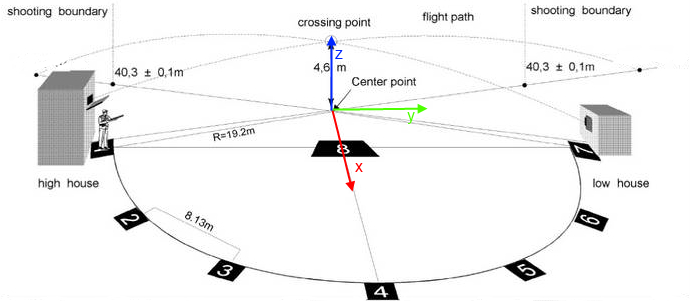
\includegraphics[width=1\textwidth]{./graphics/skeet_diagram_cropped_axes}
\caption[tekst i indholdsfortegnelsen]{figurtekst}
\label{fig:ES}
\end{figure}	
Systemets input er 60 kartesiske koordinatsæt (x ; y ; z) per sekund. Hvor de kartesiske koordinater kommer fra er uden for projektafgrænsningen. \\

I ES affyres serier af lerduer fra "High House" eller "Low House". Gennem serien skifter skytten mellem de otte stationer langs cirkelperiferien. Det kartesiske koordinatsystems origo ses på skitsen over banen, figur \ref{fig:ES}.\\

Det kartesiske koordinatsystem har origo på banens centrum. Akserne er indtegnet på figur \ref{fig:ES}. PTS's origo er placeret 45 [cm] over jorden. PTS står i udgangsposition med \(\phi\) og \(\theta\) lig med 0. Dvs. at tilts ramme står parallelt med yz-planet og det påmonteret gevær er parallelt med x-planet.\\

Geværet der bruges i ES har en spredning på ca. 2\degree. Systemet skal altså sigte efter målet med en nøjagtighed på \(\pm 1 \degree\) før geværet affyres. Ideelt set skal skytten skyde ca. når lerduen rammer toppunktet. Derfor skal PTS følge være "settlet" på lerduen inden lerduens toppunkt er nået.\\

Pans rotationen er begrænset til 170\degree\todo[author=Michael]{Mangler: Mål pan-rammens bevægelsesfrihed} omkring z-planet. Dette begrænser derved PTS maksimale overshoot.\\

Lerduen bliver affyret med en hastighed på 34,589 \([\frac{m}{s}]\) i en vinkel på \(9,103^{\circ}\) ift. xz-planet, i 3D-rummet med negligerbar luftmodstand og tyngdekraft. Set ovenfra bevæger målet sig som set på figur \ref{fig:para_in_xy_plane}. 
På figur \ref{fig:HH2D_para} ses nedslagspunktet, G, fra High-House 52 [m] efter startpositionen, D, samt  
PTS placering i punktet B.\\
\begin{figure}[h!]
\centering
\subfloat[Lerduens højde som funktion af afstanden.\label{fig:HH2D_para}]{%
	\begin{tikzpicture}[scale=0.8]
	\include*{./graphics/high_house_2D_parabola}
	\end{tikzpicture}
}
\subfloat[Lerduens bane projekteret på xy-planet.\label{fig:para_in_xy_plane}]{%
	\begin{tikzpicture}[scale=0.16]
	\include*{./graphics/parabola_in_xy_plane}
	\end{tikzpicture}
}
\caption[Lerduens parabel i 2D]{Viser parablen af lerduens bane i 2D.}
\end{figure}

PTS dimensioneres til en konkurrence i ES og er afgrænset til et enkelt tilfælde: Afskydning fra ”High-House” med PTS placeret på station 4. Øvrige kravspecificeringer fåes i sektion \ref{sec:kravspecifikation}.